\section{\uppercase{3D scene modeling}}\label{sec:modeling}

\noindent For being able to compute the surface coverage of a given set of simulated target objects that a given constellation of sensors can observe, it is necessary to model the 3D geometry of the scene objects. Moreover, the depth sensors must have a realistic data acquisition model that is representative of the real sensors. As such, the development of the proposed system started with the 3D modeling of the scene geometry, namely the environment objects and sensors 3D models using \gls{cad} systems. Later on, several types of depth sensors were modeled within the Gazebo simulator\footnote{\url{http://gazebosim.org}} in order to perform accurate 3D rendering of the scene and generate representative sensor data taking into consideration the specific characteristics of each type of sensor (such as image resolution, field of view and depth range) while also accounting for the occlusions that other objects in the environment might cause in relation to the target models that each sensor is trying to observe from its given view point. The next sections will present the modeling of the simulation worlds along with how the depth sensors were deployed within plausible regions of interest that take into account where the sensors can be placed in the real environment.


\subsection{\uppercase{Environment modeling}}

For testing active perception and bin picking operations it was modeled 4 different simulation worlds. Within these environments it was deployed one or several target objects (which was a starter motor \gls{cad} model with a unique green surface material that had no light effects, such as shading and shadows). The first environment (shown in \cref{fig:active-perception-environment}), focused on an active perception task in which a starter motor was placed on top of a trolley and was being occluded by a human hand starting to grasp it. The goal of this environment was to simulate an active perception task, in which we may need to actively move a sensor within the environment to be able to keep tracking the pose of a given object (such is the case of objects that are being manipulated by humans in which the hands are creating significant occlusions and a static sensor constellation may not be able to observe enough surface geometry to be able to perform pose tracking with accuracy). On the other 3 worlds, the main goal was similar but applied to bin picking operations. In this use case a static overhead camera can provide a rough estimation of the target objects and then based on the level of object recognition confidence and how significant are the occlusions, we may need to move a sensor attached to a robotic arm to several positions in order to gather further sensor data to increase the object recognition confidence and its pose estimation accuracy. In the first bin picking world, the starter motor was inside a large staking box together with an alternator and a gearbox (displayed in \cref{fig:bin-picking-environment}). The second bin picking environment is a variation of the first in which it was added 3 more differential gearboxes into the stacking box in order to significantly increase the occlusion of the target object (seen in \cref{fig:bin-picking-with-occlusions-environment}). Finally, the last bin picking environment (seen in \cref{fig:multiple-bin-picking-with-occlusions-environment}) is another variation of the first environment in which it was added 3 more target objects (one on top of the trolley and two on the its middle shelves).

\begin{figure}
	\centering
	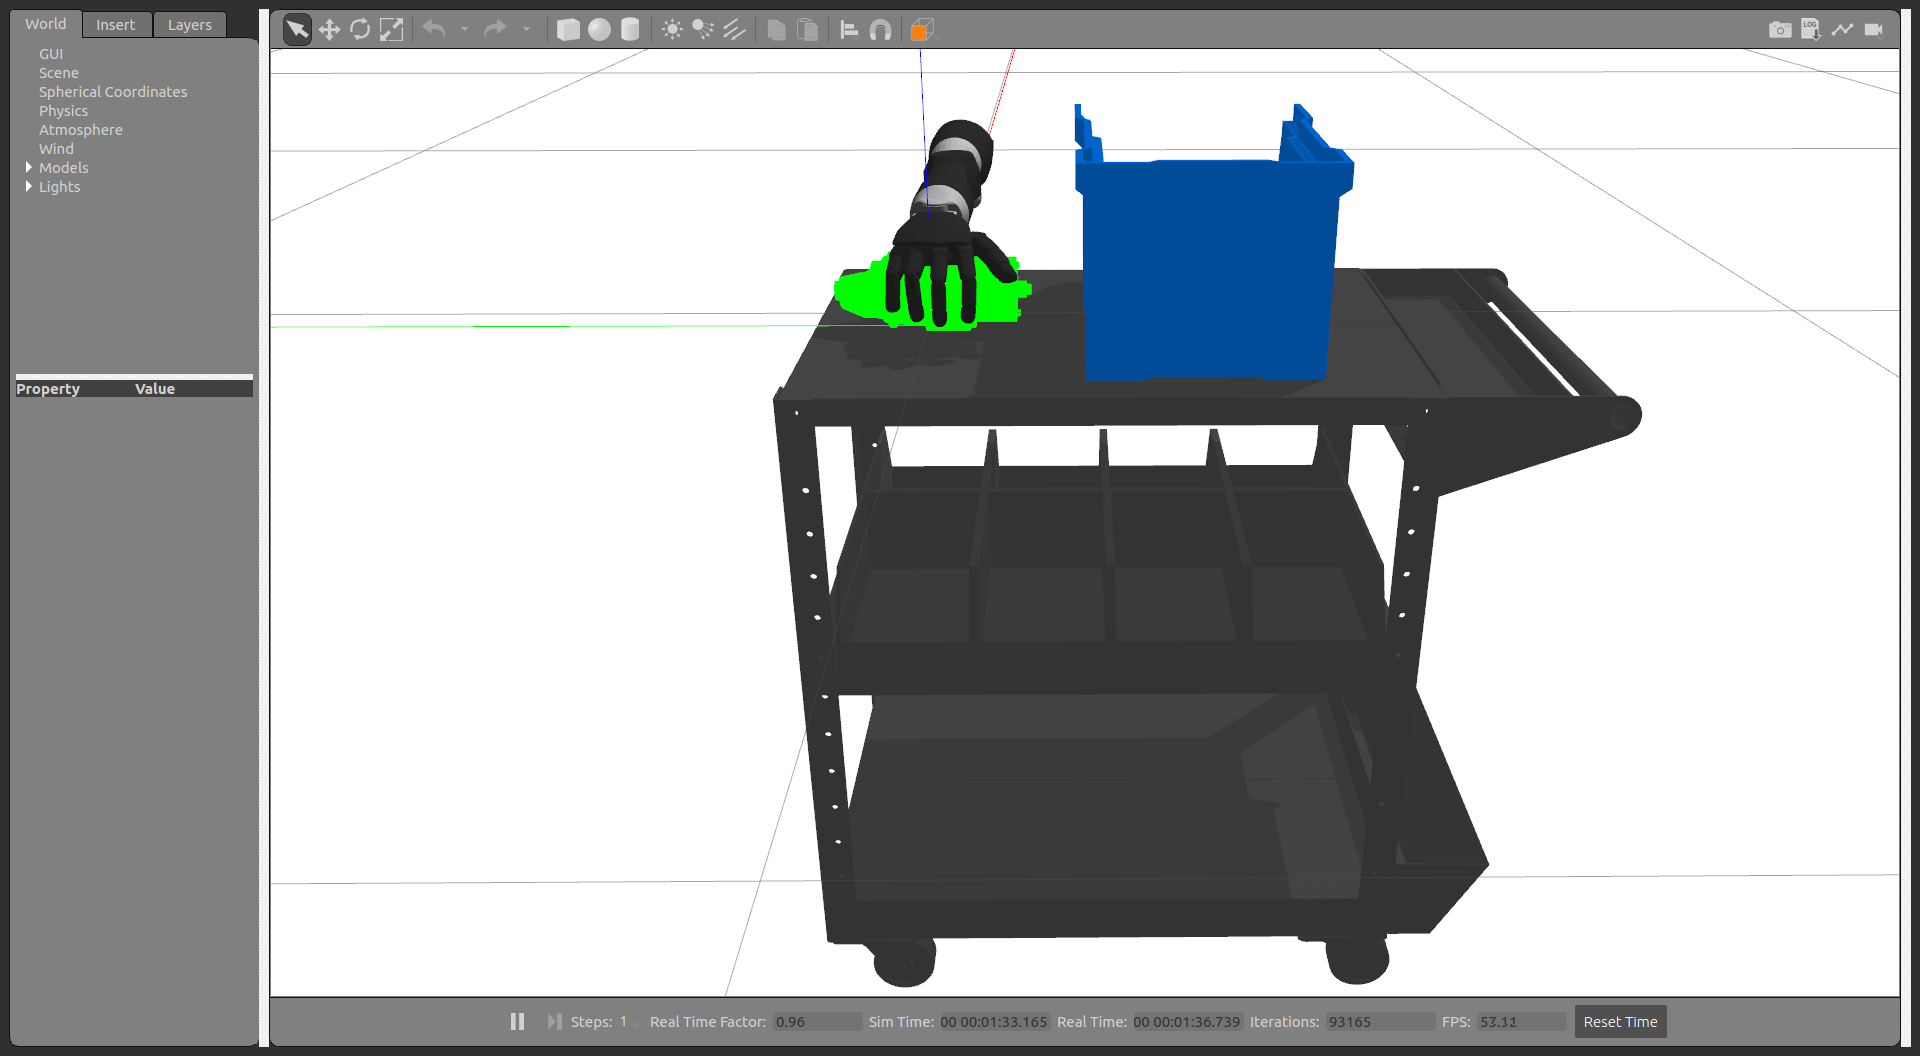
\includegraphics[height=.126\textwidth]{environments/active-perception/gazebo-back}
	\includegraphics[height=.126\textwidth]{environments/active-perception/gazebo-top}\\
	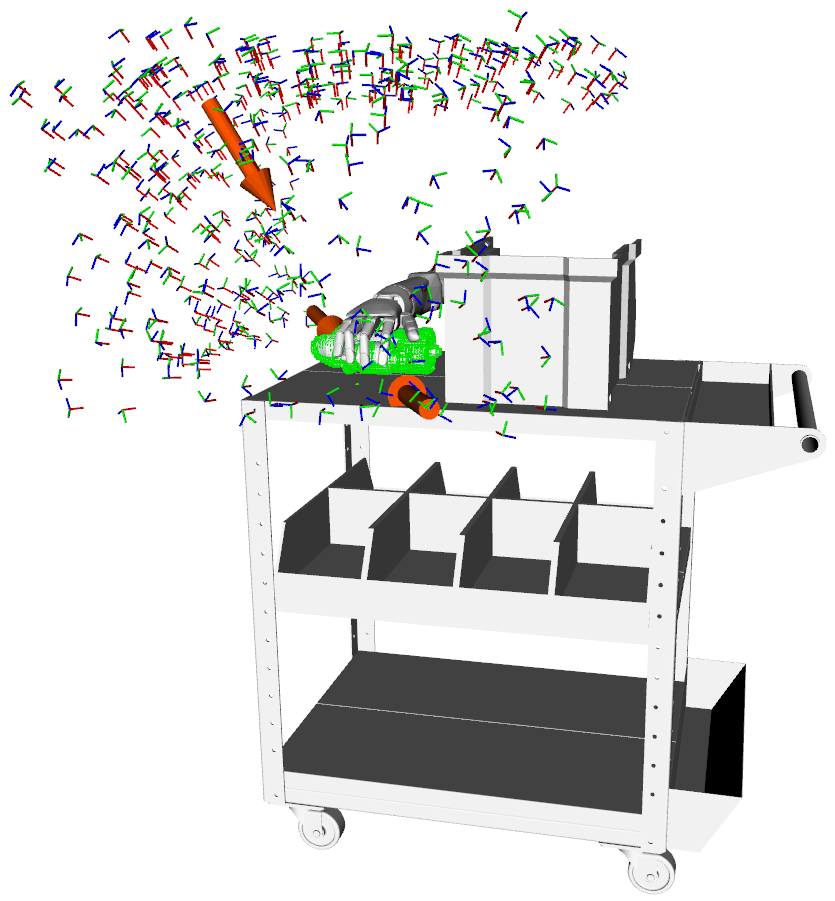
\includegraphics[height=.126\textwidth]{environments/active-perception/rviz-back-left}
	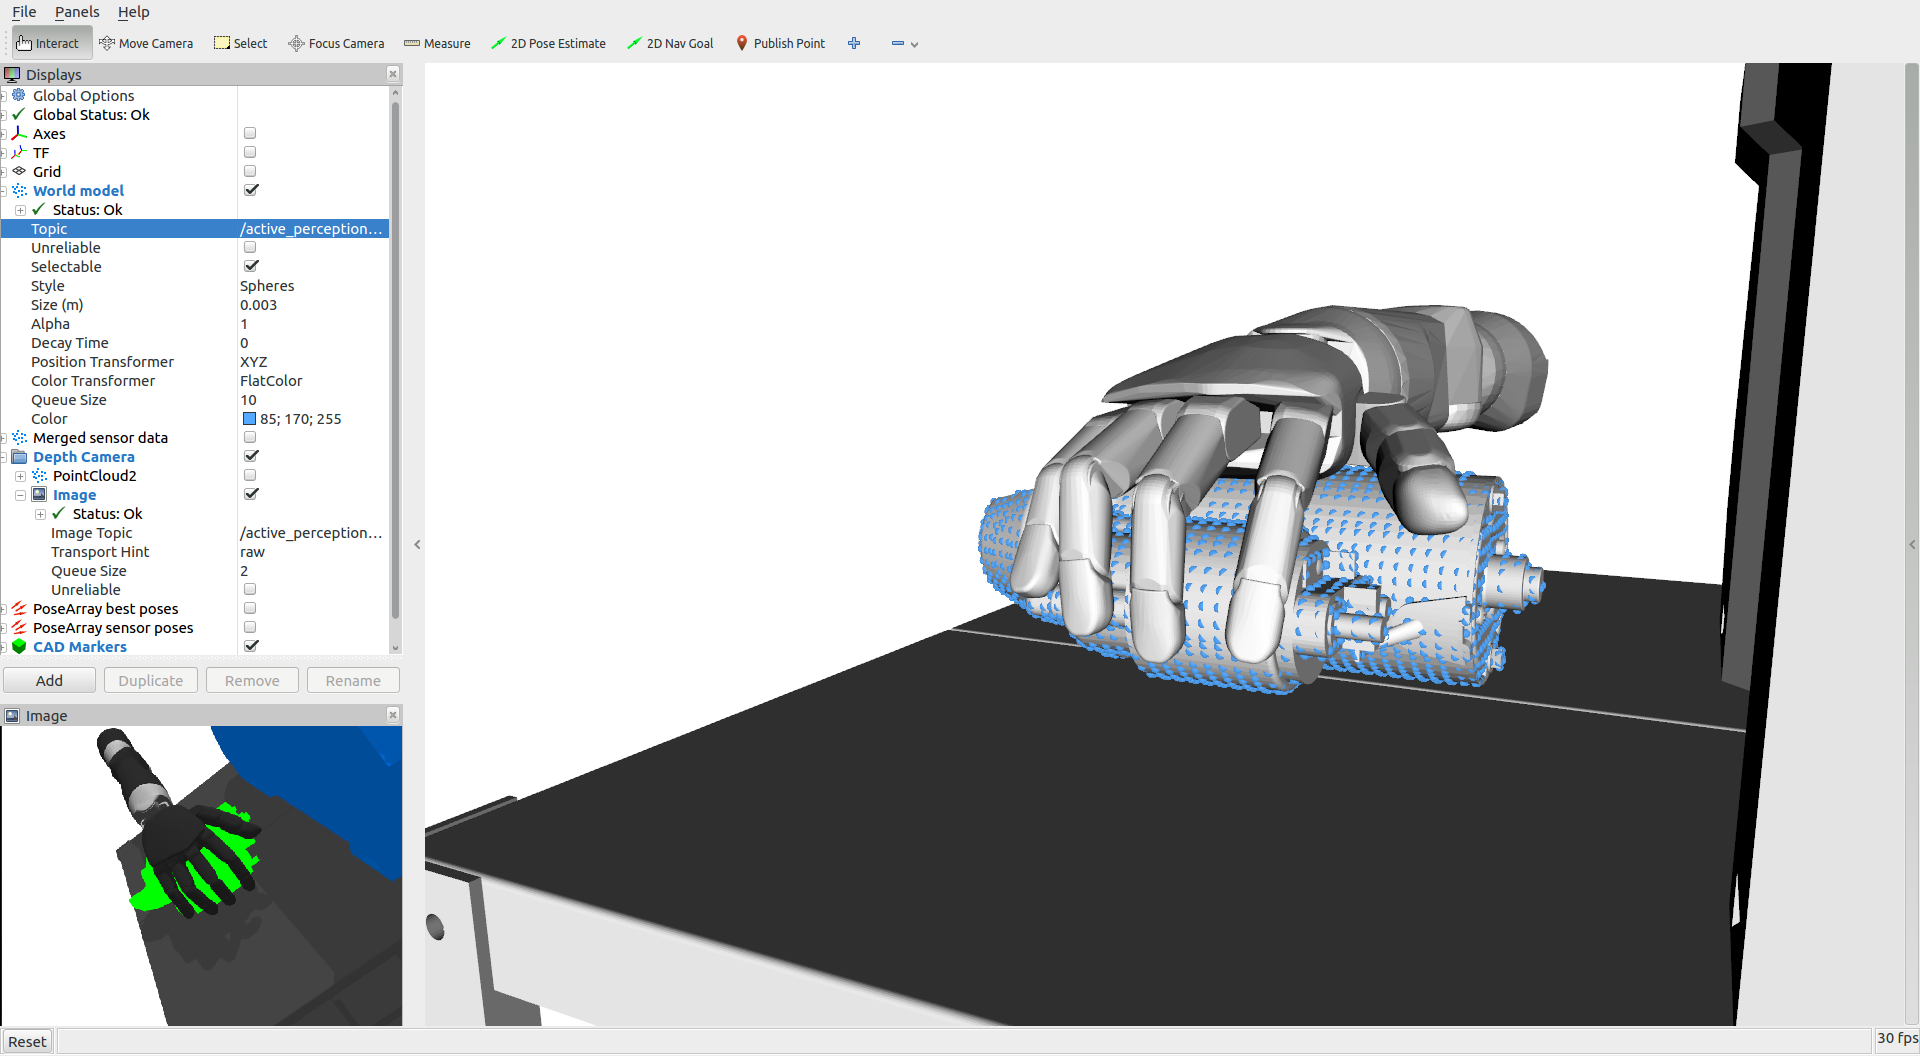
\includegraphics[height=.126\textwidth]{environments/active-perception/rviz-back-right}
	\caption{Active perception environment renderings from Gazebo with target objects in green (top images) and associated CAD model point clouds displayed as blue spheres in Rviz (bottom images)}
	\label{fig:active-perception-environment}
\end{figure}

\begin{figure}
	\centering
	\includegraphics[height=.126\textwidth]{environments/bin-picking/gazebo-front}
	\includegraphics[height=.126\textwidth]{environments/bin-picking/gazebo-top}\\
	\includegraphics[height=.126\textwidth]{environments/bin-picking/rviz-front}
	\includegraphics[height=.126\textwidth]{environments/bin-picking/rviz-top}
	\caption{Bin picking environment renderings from Gazebo with target objects in green (top images) and associated CAD model point clouds displayed as blue spheres in Rviz (bottom images)}
	\label{fig:bin-picking-environment}
\end{figure}

\begin{figure}
	\centering
	\includegraphics[height=.126\textwidth]{environments/bin-picking-with-occlusions/gazebo-front}
	\includegraphics[height=.126\textwidth]{environments/bin-picking-with-occlusions/gazebo-top}\\
	\includegraphics[height=.126\textwidth]{environments/bin-picking-with-occlusions/rviz-front}
	\includegraphics[height=.126\textwidth]{environments/bin-picking-with-occlusions/rviz-top}
	\caption{Bin picking with occlusions environment renderings from Gazebo with target objects in green (top images) and associated CAD model point clouds displayed as blue spheres in Rviz (bottom images)}
	\label{fig:bin-picking-with-occlusions-environment}
\end{figure}

\begin{figure}
	\centering
	\includegraphics[height=.126\textwidth]{environments/multiple-bin-picking-with-occlusions/gazebo-front}
	\includegraphics[height=.126\textwidth]{environments/multiple-bin-picking-with-occlusions/gazebo-top}\\
	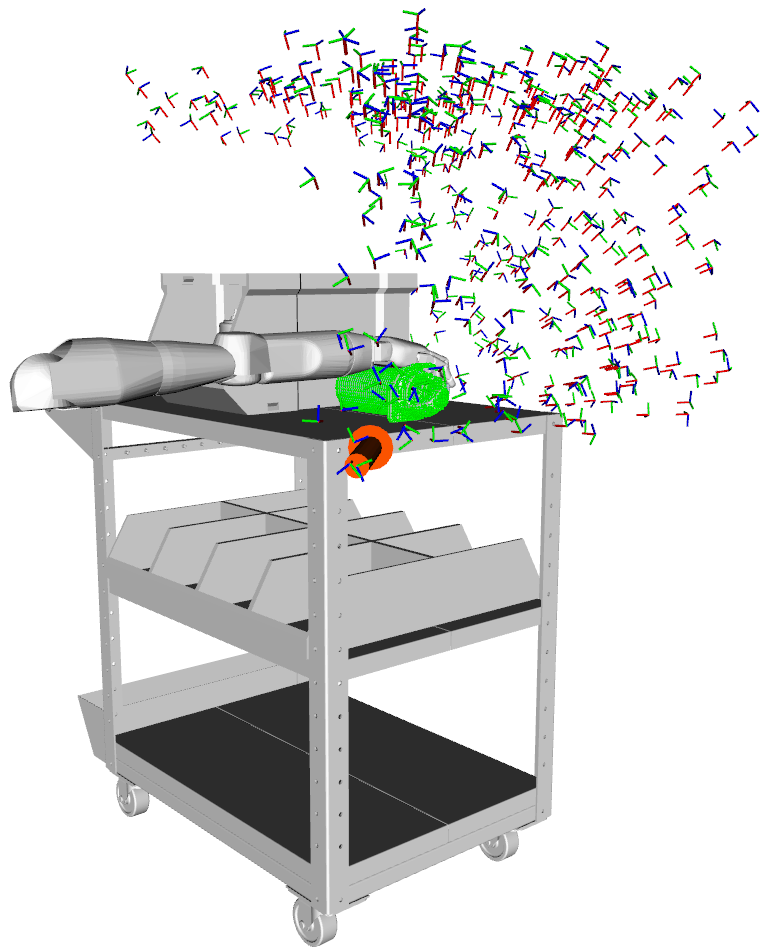
\includegraphics[height=.126\textwidth]{environments/multiple-bin-picking-with-occlusions/rviz-front-corner}
	\includegraphics[height=.126\textwidth]{environments/multiple-bin-picking-with-occlusions/rviz-top}
	\caption{Multiple bin picking with occlusions environment renderings from Gazebo with target objects in green (top images) and associated CAD model point clouds displayed as blue spheres in Rviz (bottom images)}
	\label{fig:multiple-bin-picking-with-occlusions-environment}
\end{figure}


\subsection{\uppercase{Sensors modeling}}

Over the years it was developed a wide range of technologies for performing environment sensing. From the passive image sensors to the active systems that probe the environment using projected patterns, lasers or \gls{tof} devices. Given that the goal of the proposed system was to perform active perception or environment monitoring, it was modeled 8 different types of depth sensors (shown in \cref{fig:sensors}) which relied on 3 types of environment sensing technologies. One of them was the Kinect XBox One \gls{tof} device, 5 were structured light sensors (such as the Asus Xtion Pro Live, the Ensenso N35, the Intel RealSense SR300, the Kinect XBox 360 and the Orbbec Astra) and 2 were stereo vision systems (namely the MultiSense S7 and the ZED stereo camera). Each of these depth sensors can be modeled using the pinhole camera model, which allows to specify the main unique characteristics of each sensor, such as the depth image resolution (width and height in pixels), its \gls{fov} (horizontal and vertical in radians) and the range in which the sensor can retrieve valid measurements (minimum and maximum in meters). Moreover, since this camera model is implemented in most 3D rendering engines and optimized in todays powerful \glspl{gpu}, the sensor data generation can be performed very fast and efficiently using 3D rendering \glspl{api} such as the \gls{opengl}. This is the case of the Gazebo simulator, that uses the Ogre3D\footnote{\url{http://www.ogre3d.org}} rendering engine which in turn relies on \gls{opengl}. Besides camera modeling, Gazebo also allows to simulate the sensor acquisition rate (specified as the number of depth images generated per second), which is usually higher on structured light sensors and lower on stereo vision systems.

\begin{figure}
	\centering
	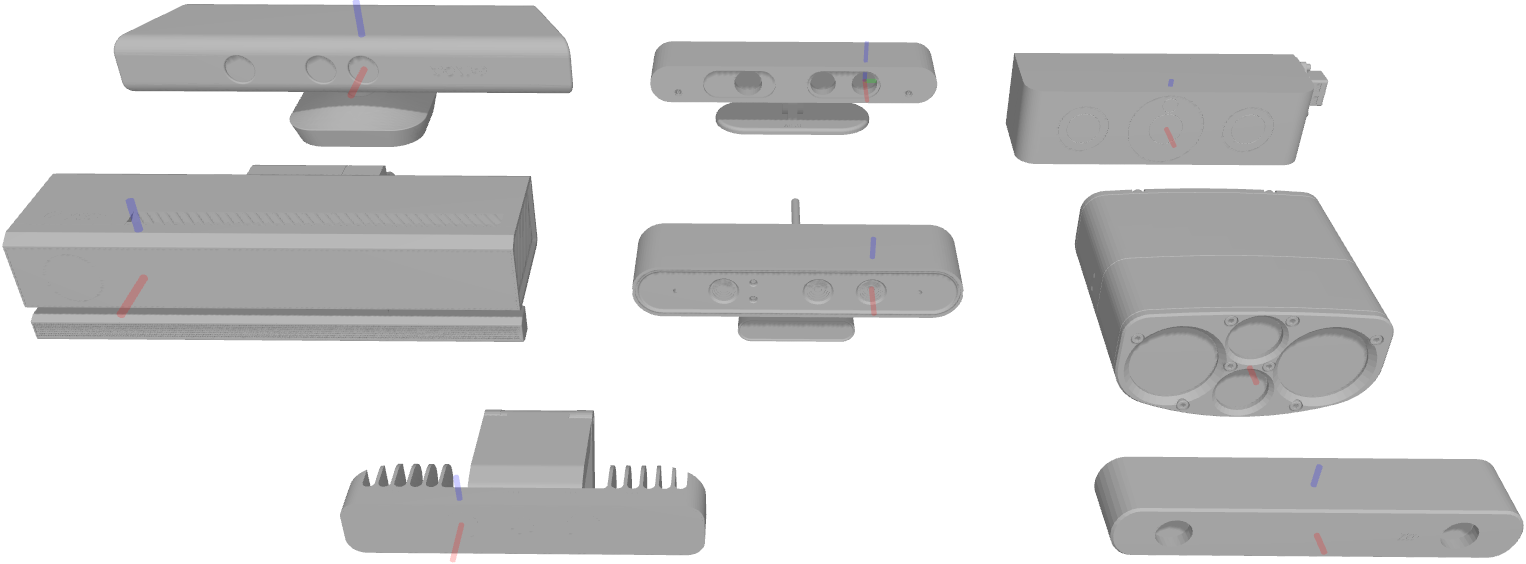
\includegraphics[width=.47\textwidth]{sensors/sensors-gray-with-links}
	\caption{Sensors 3D CAD models with the display of the depth image coordinate frames using the ROS convention of x-y-z -> forward-left-up (horizontally from top left to bottom right: Kinect XBox 360, Asus Xtion Pro Live, Ensenso N35, Kinect XBox One, Orbbec Astra, MultiSense S7, Intel RealSense SR300, ZED stereo camera)}
	\label{fig:sensors}
\end{figure}


\subsection{\uppercase{Sensors deployment}}\label{subsec:sensors-deployment}

Implementation text.

\begin{itemize}
	\item For making the estimation of the sensor disposition computational feasible, the 3D continuous space was populated with a given set of sensors that were looking at a given point (with the sensor roll either 0º or random)
	\item Several populations of sensors can be added to the world
	\begin{itemize}
		\item The 3D sensor models will be hidden at rendering time to avoid occlusion of sensor data
	\end{itemize}
	\item Each population is of a given sensor type and is deployed within a given region of interest 
	\begin{itemize}
		\item This allows to restrict the spatial distribution of the sensors, for example a given set of sensors should be in the walls or ceiling due to their weight, or they should be close to the target object given their limited depth measurements range
	\end{itemize}
	\item Currently supported deployment configurations:
	\begin{itemize}
		\item Uniform or random deployment within a box
		\item Uniform or random deployment within a cylinder
		\item Uniform within a 2D grid (with a set of rows and columns)
		\item Uniform along a line
	\end{itemize}
\end{itemize}

\begin{itemize}
	\item For the active perception environment, 450 sensors were deployed close to the target object, on the top, right and back side of the trolley
	\item This was done to simulate the closest range in which a dynamically moving sensor attached to a robotic arm could move (taking into consideration the human safety and the sensor minimum measurement distance, that was 0.2 meters)
\end{itemize}
\begin{figure}
	\centering
	\includegraphics[height=.22\textwidth]{sensor-deployment/active-perception/gazebo-front}\hspace{1em}
	\includegraphics[height=.22\textwidth]{sensor-deployment/active-perception/gazebo-top}
	\caption{Sensors deployment on the active perception environment}
\end{figure}


\begin{itemize}
	\item For the single bin picking environments, given that the target object was inside the stacking box, the sensors were deployed close to the target object, but only on top of the trolley, on 3 layers (each with a different type of sensor).
	\item In the world with minimal occlusions it was deployed 100 sensors while in the world with significant occlusions it was deployed 300 sensors
	\begin{itemize}
		\item The sensor density was increased given that the best views have tighter observation regions which could be missed with a sparse sensor deployment
	\end{itemize}
\end{itemize}
\begin{figure}
	\centering
	\includegraphics[height=.29\textwidth]{sensor-deployment/bin-picking/gazebo-sensors}\hspace{1em}
	\includegraphics[height=.29\textwidth]{sensor-deployment/bin-picking-with-occlusions/gazebo-sensors}
	\caption{Sensors deployment on the single bin picking environments}
\end{figure}

\begin{itemize}
	\item For the multiple bin picking environment, given that there were multiple target objects (1 inside the stacking box, 1 on top and 2 on the shelves of the trolley), it was deployed 450 sensors across 7 populations:
	\begin{itemize}
		\item 5 populations simulating fixed sensors on the walls and ceiling
		\item 2 populations above the trolley, simulating dynamic sensors attached to a robotic arm
	\end{itemize}
\end{itemize}
\begin{figure}
	\centering
	\includegraphics[height=.164\textwidth]{sensor-deployment/multiple-bin-picking-with-occlusions/gazebo-front}\hspace{1em}
	\includegraphics[height=.164\textwidth]{sensor-deployment/multiple-bin-picking-with-occlusions/gazebo-top}
	\caption{Sensors deployment on the multiple bin picking environment}
\end{figure}
